%enemies.tex
Here a list of all enemies with a short description is given. Enemies information are obtained from: 
\begin{itemize}
	\item X1: \cite{wayback:X_resources},\cite{wiki:X1_enemies},
	\item X2: \cite{wayback:X2_resources},\cite{wiki:X2_enemies}
\end{itemize}
while all artworks come from \cite{book:MMX_Complete_art}. In some occasions artworks from the X Dive game will also  be shown.

%TODO RAPPORTARE NEMICI X2 SECONDO 3 DANNI PER COLPO

\section{Mini-Bosses}
\begin{itemize}
	\item \hypertarget{miniboss:Anglerge}{\textbf{Anglerge}}:
	\enemSpecs{64 (0.15 seconds of Iframe, Boomerang Cutter, Sting Chameleon and Rolling Shields hit for 8 damage) }{4 (contact), 2 (snakes)}{Angler-type mechaniloids that work to cleaning the seabed floor, with a motion sensor attached to its "lantern" part.}
	\begin{figure}[htp]
		\centering
		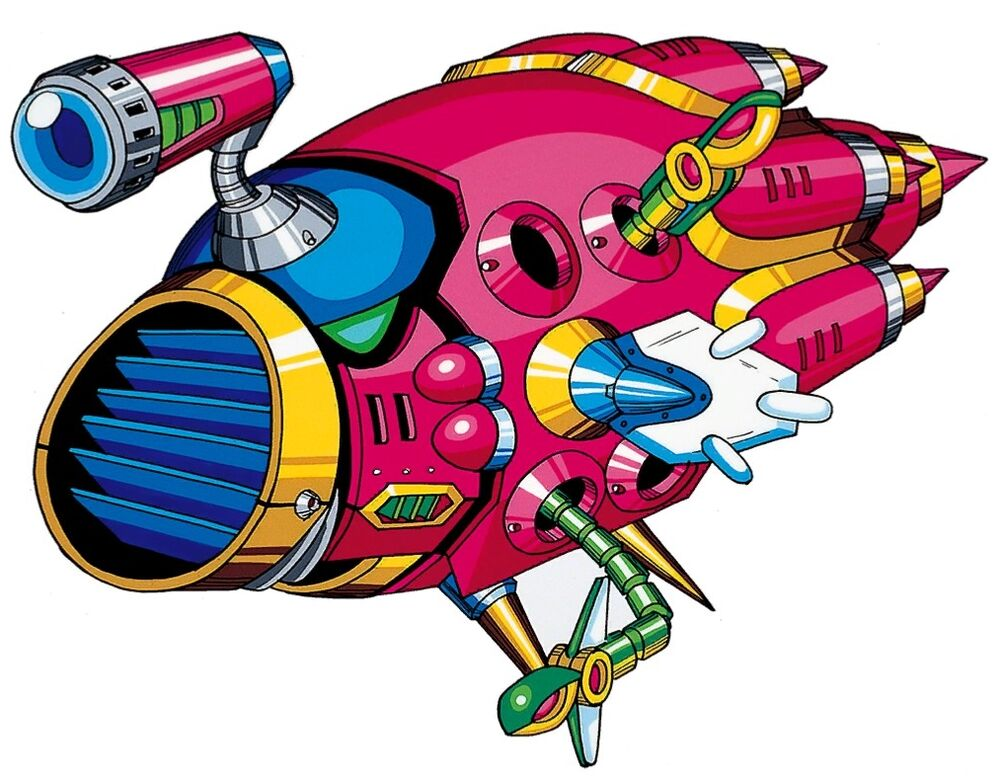
\includegraphics[width=0.35\linewidth]{figures/X1/Enemies/Anglerge.jpg}
		\caption{Anglerge's artwork}
	\end{figure}
	
	\item \hypertarget{miniboss:Bee_Blader}{\textbf{Bee Blader}}:
	\enemSpecs{32 (No Iframes)}{4 (contact), 2 (missiles), 1 (machine gun)}{A large bee-type helicopter which was created in order to carry \hyperlink{enem:Ball_De_Voux}{Ball de Voux}. It is equipped with a vulcan machine-gun and homing missiles. This mechaniloid has been created for guerrilla operations in forests and cities. While they don't appear formidable enemies, they can be rather dangerous, especially if X defeats them while standing below, as they will fall and crush him instantly.}
	\begin{figure}[htp]
		\centering
		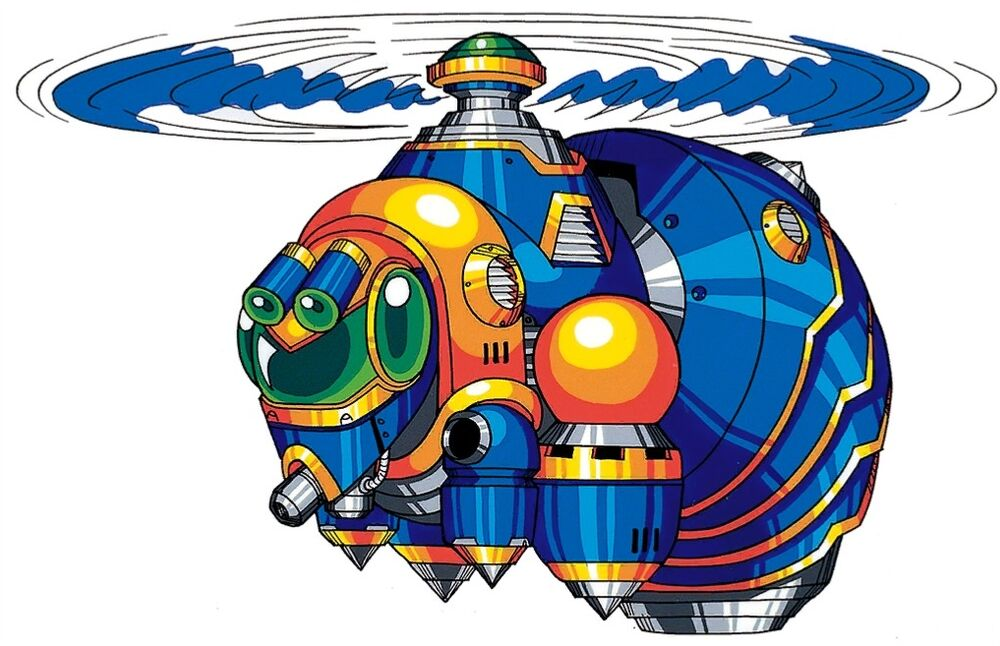
\includegraphics[width=0.4\linewidth]{figures/X1/Enemies/BeeBlader.jpg}
		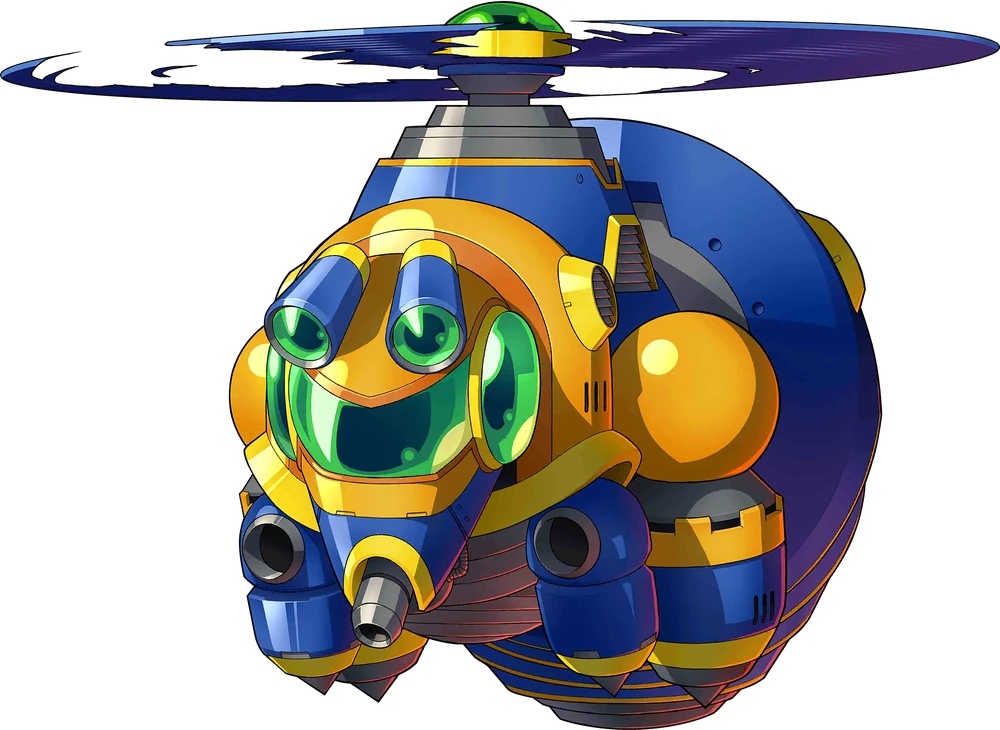
\includegraphics[width=0.4\linewidth]{figures/X1/Enemies/BeeBlader_Dive.png}
		\caption{Bee Blader's artworks}
	\end{figure}
	
	\item \hypertarget{miniboss:Chop_Register}{\textbf{Chop Register}}
	\enemSpecs{32 (weak only in the handle, a Giga Crush or a well-placed charged Sonic Slicer one shots it)}{2 (contact)}{Sigma Virus substantiated into the form of a sword. Its patterns are based on Sigma's own saber skill.}
	\begin{figure}[htp]
		\centering
		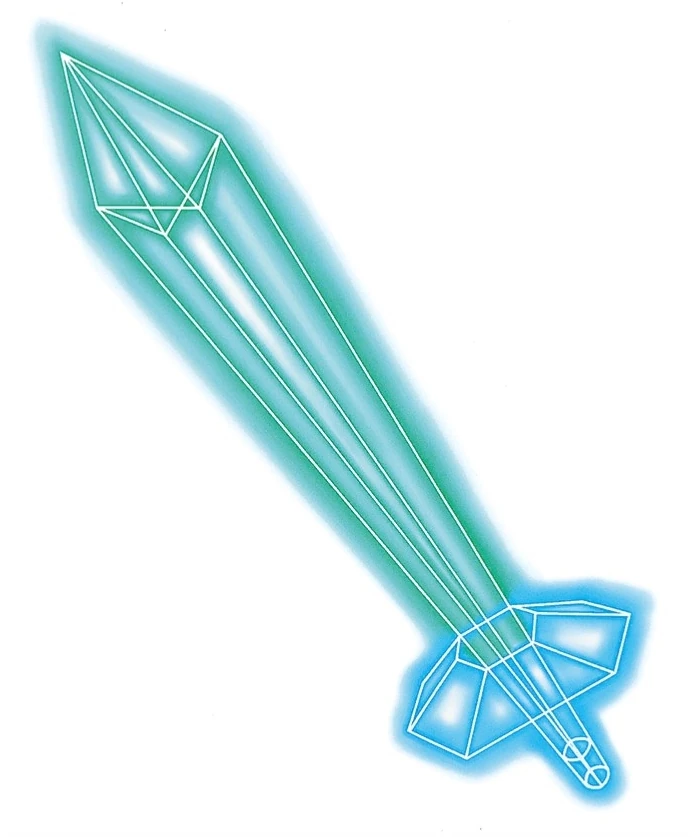
\includegraphics[width=0.33\linewidth]{figures/X2/Enemies/ChopRegister.png}
		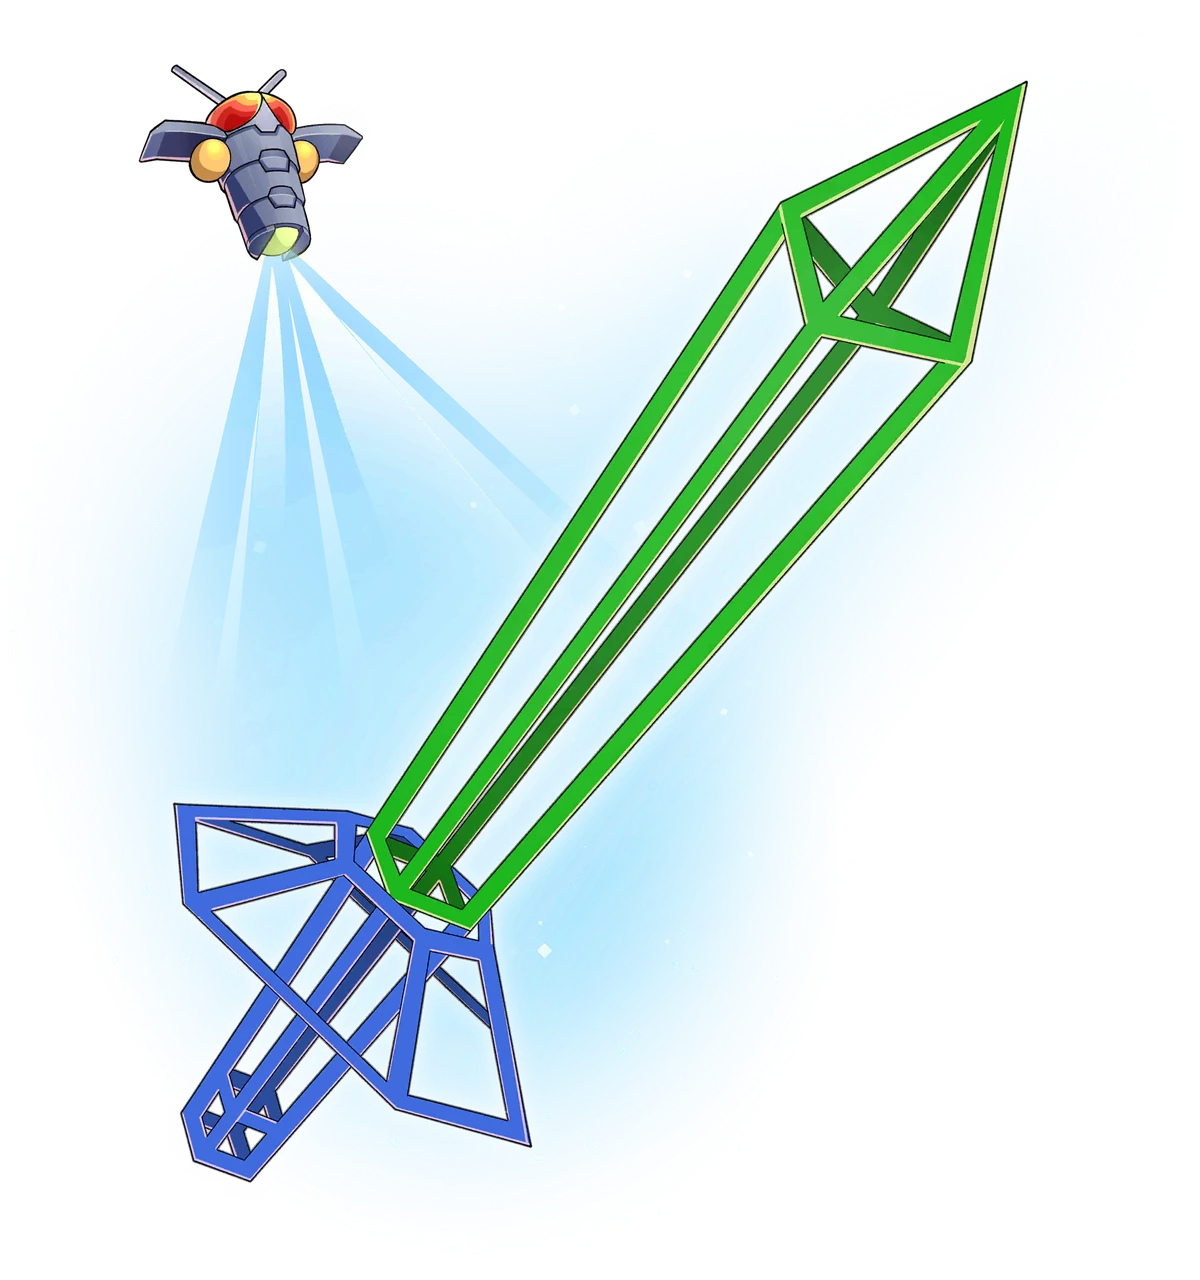
\includegraphics[width=0.33\linewidth]{figures/X2/Enemies/ChopRegister_Dive.png}
		\caption{Chop Register's artworks }
	\end{figure}

	\item \hypertarget{miniboss:Cruiziler}{\textbf{Cruiziler}}: 
	\enemSpecs{64 (resist most weapons but no Iframes, meaning a Storm Tornado is a guaranteed kill)}{3 (bombs)}{Whale mechaniloid who patrols the sea with its powerful weapon. Some kind of mistake caused it to lose its sea navigation, its attack circuits began running wild, and communications were lost. Its body is totally invincible, save for its core on top.}
	\begin{figure}[htp]
		\centering
		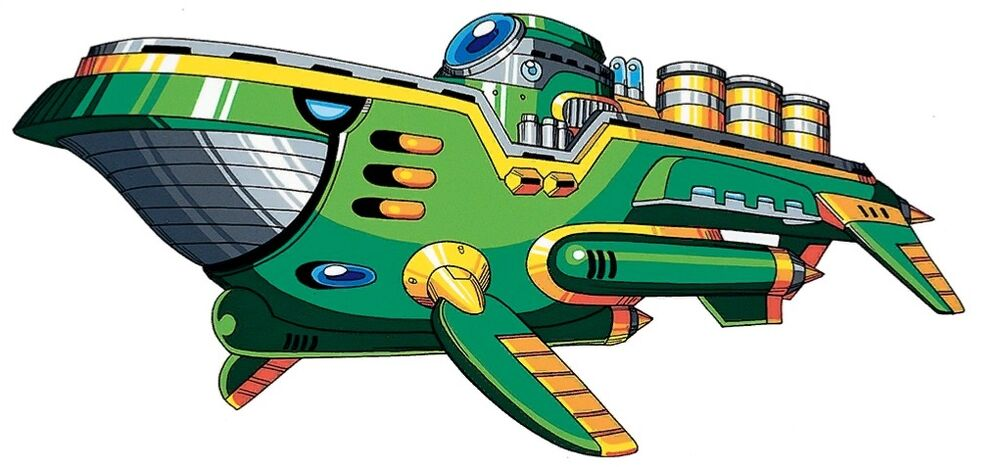
\includegraphics[width=0.55\linewidth]{figures/X1/Enemies/Cruiziller.jpg}
		\caption{Cruiziller's artwork}
	\end{figure}

	\item \hypertarget{miniboss:Genjibo}{\textbf{Genjibo}} 
	
	\item 
	\hypertarget{miniboss:Hotareeca}{\textbf{Hotareeca}}
	
	\item \hypertarget{miniboss:Magna_Quartz}{\textbf{Magna Quartz}}
	\enemSpecs{20 (~0.97 seconds of Iframes, weak to silk shot)}{2 (contact with laser shooters), 2 (laser), 3 (contact with crystal)}{An unknown mechaniroid, embedded in a giant crystal. Attacks using 2 invincible support mechas, which fire reflecting lasers. Its true form inside the crystal is its weakness.}
	\begin{figure}[htp]
		\centering
		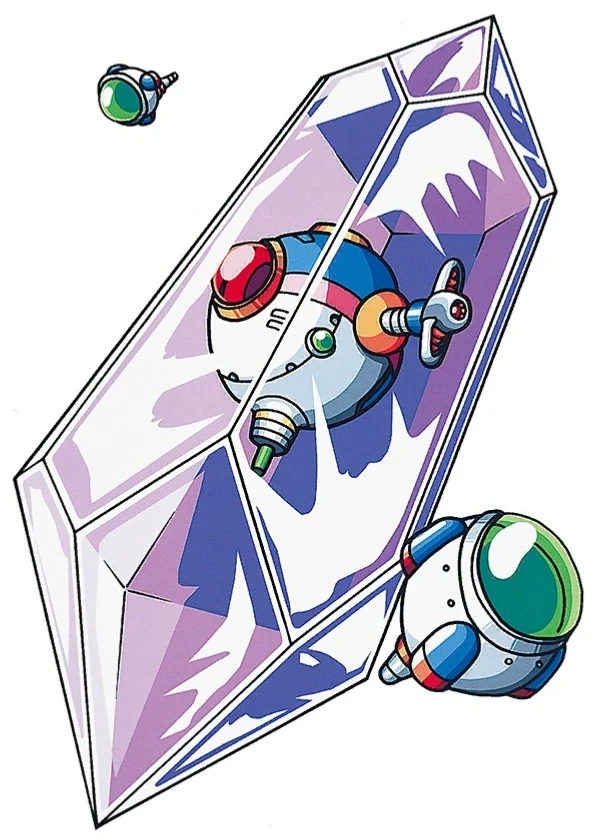
\includegraphics[width=0.3\linewidth]{figures/X2/Enemies/MagnaQuartz.png}
		
\includegraphics[width=0.25\linewidth]{figures/X2/Enemies/MagnaQuartz_Dive.png}
		\caption{Magna Quartz's artworks }
	\end{figure}
		
	\item \hypertarget{miniboss:Mole_Borer}{\textbf{Mole Borer}}:
	\enemSpecs{60 ($\sim$0.083 seconds of Iframes. Fire Wave deals 3 damage each 2 frames)}{Insta-kill (roller), 2 (contact)}{Mechanioid used to open up paths in mines, using a rotary roller to destroy rocks that obstruct his path. Its armoring can take a lot of damage, while the roller is completely invincible and can instantly kill X. The only way to deal with it is to attack from behind, although several shots are needed to take it down. Using the Fire Wave is the best option, as its continuous damage can dispose of it quickly.}
	\begin{figure}[htp]
		\centering
		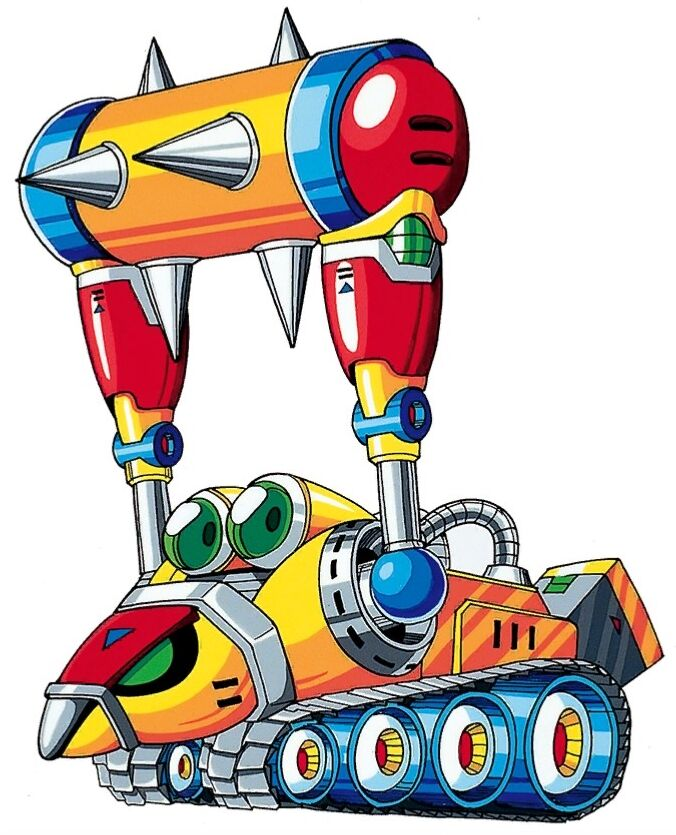
\includegraphics[width=0.3\linewidth]{figures/X1/Enemies/MoleBorer.jpg}
		
\includegraphics[width=0.3\linewidth]{figures/X1/Enemies/MoleBorer_Dive.png}
		\caption{Mole Borer's artworks}
	\end{figure}

	\item \hypertarget{miniboss:Old_robot}{\textbf{Old Robot}}
	\enemSpecs{10, weak to Silk Shot, Magnet Mine and Spin Wheel. A well placed charged Spin Wheel or Silk shot one-shots it. Resurrect if the \hyperlink{miniboss:Pararoid_S-38}{Pararoid S-38} is not defeated quickly}{2 (scrap shot), 2 (contact)}{Combat robot used in wars of the past. Heavily armored, attacks were once useless on this invincible robot, but with the end of the wars, it was turned to scrap.}
	\begin{figure}[htp]
		\centering
	\begin{subfigure}{0.6\linewidth}
		
\includegraphics[width=0.49\linewidth]{figures/X2/Enemies/OldRobot.png}
		
\includegraphics[width=0.49\linewidth]{figures/X2/Enemies/OldRobot_Dive.png}
	\end{subfigure}		
	\begin{subfigure}{0.2\linewidth}
		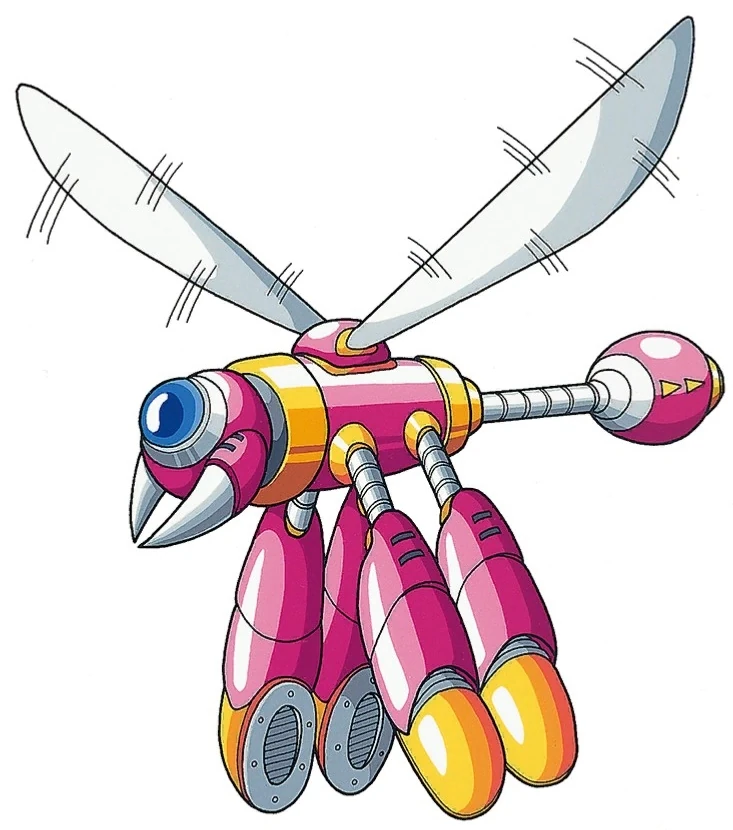
\includegraphics[width=\linewidth]{figures/X2/Enemies/PararoidS38.png}
	\end{subfigure}
		\caption{Old Robot and Pararoid S-38's artwork}

	\end{figure}
	
	\item \hypertarget{miniboss:Pararoid_S-38}{\textbf{Pararoid S-38}} 
	\enemSpecs{12, instantly killed by Sonic Slicer, Speed Burner and Giga Crush}{2 (contact)}{Next generation \hyperlink{enem:Pararoid_V-1}{Paraloid} prototype. Equipped with the ability of flight and improved durability, it posses the \hyperlink{miniboss:Old_robot}{Old Robot}, controlling it completely.}
%	\begin{figure}[htp]
%		\centering
%		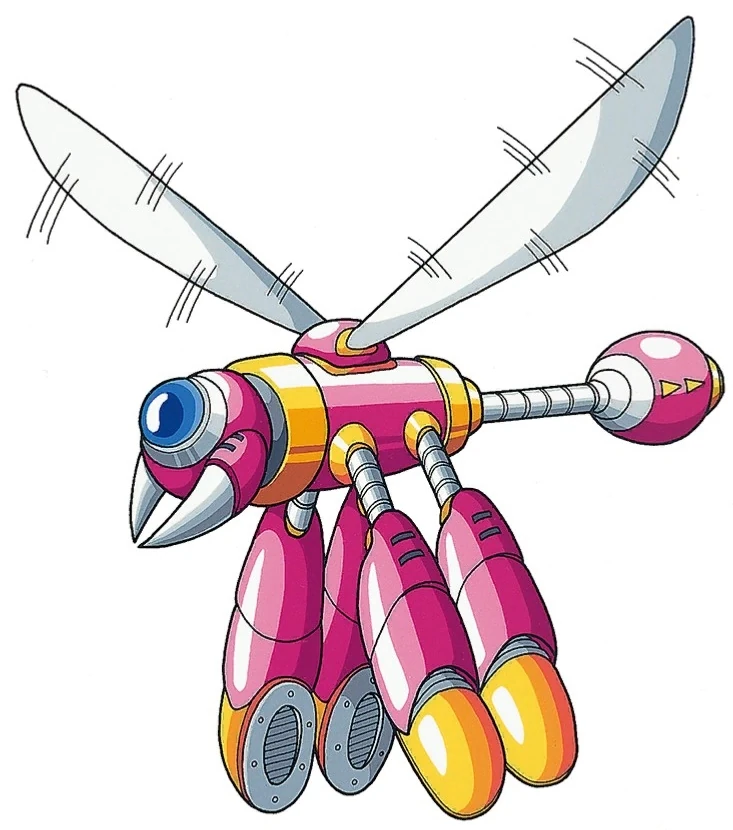
\includegraphics[width=0.2\linewidth]{figures/X2/Enemies/PararoidS38.png}
%		\caption{Paraloid S-38's artwork}
%	\end{figure}
	
	\item \hypertarget{miniboss:Raider_Killer}{\textbf{Raider Killer}}
	\enemSpecs{32 in all forms (0.5 seconds of Iframe,, Speed Burner deal 3-6 damages)}{2 (hand cannon), 3 (scatter shots), 4 (contact), 2 (shield)}{Extra-large sized private intruder (Raider) repulsion mechaniroid. When it searches an enemy with its radar, it scans the enemy's conduct patterns as well. When the radar discovers an enemy, Raider Killer's form is strengthened with a blue energy, and it enters a violent rage.}
	\begin{figure}[htp]
		\centering
		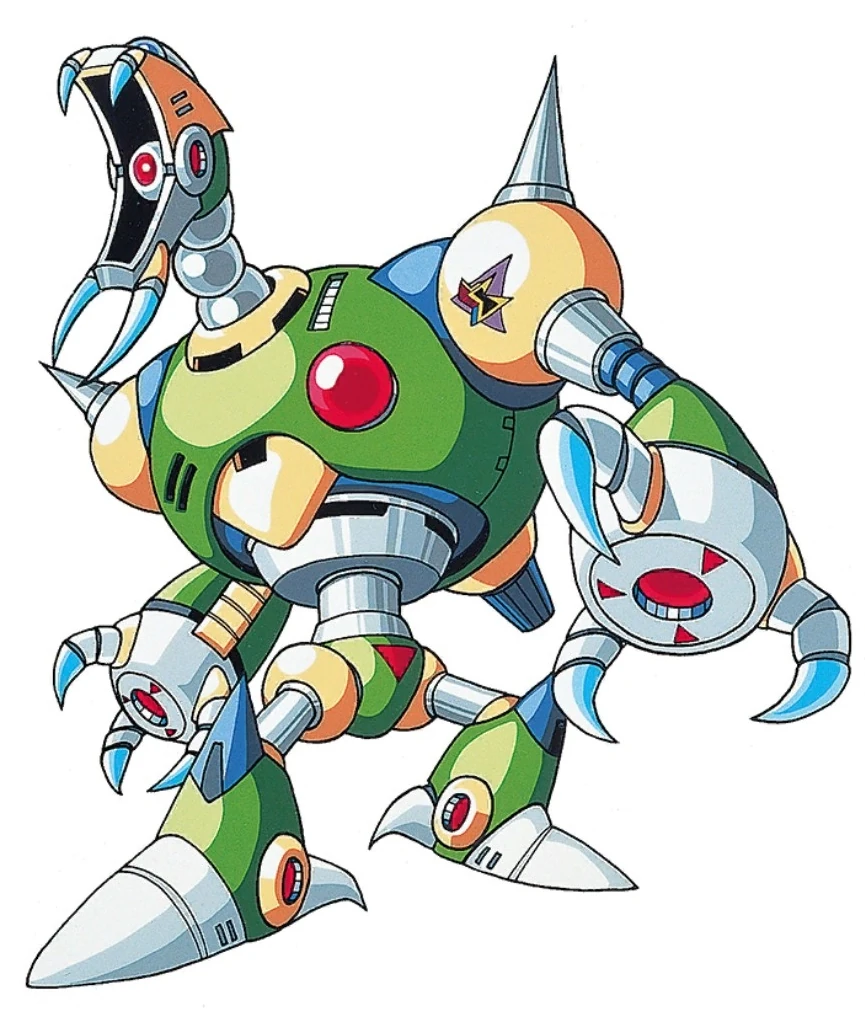
\includegraphics[width=0.3\linewidth]{figures/X2/Enemies/RaiderKiller.png}
		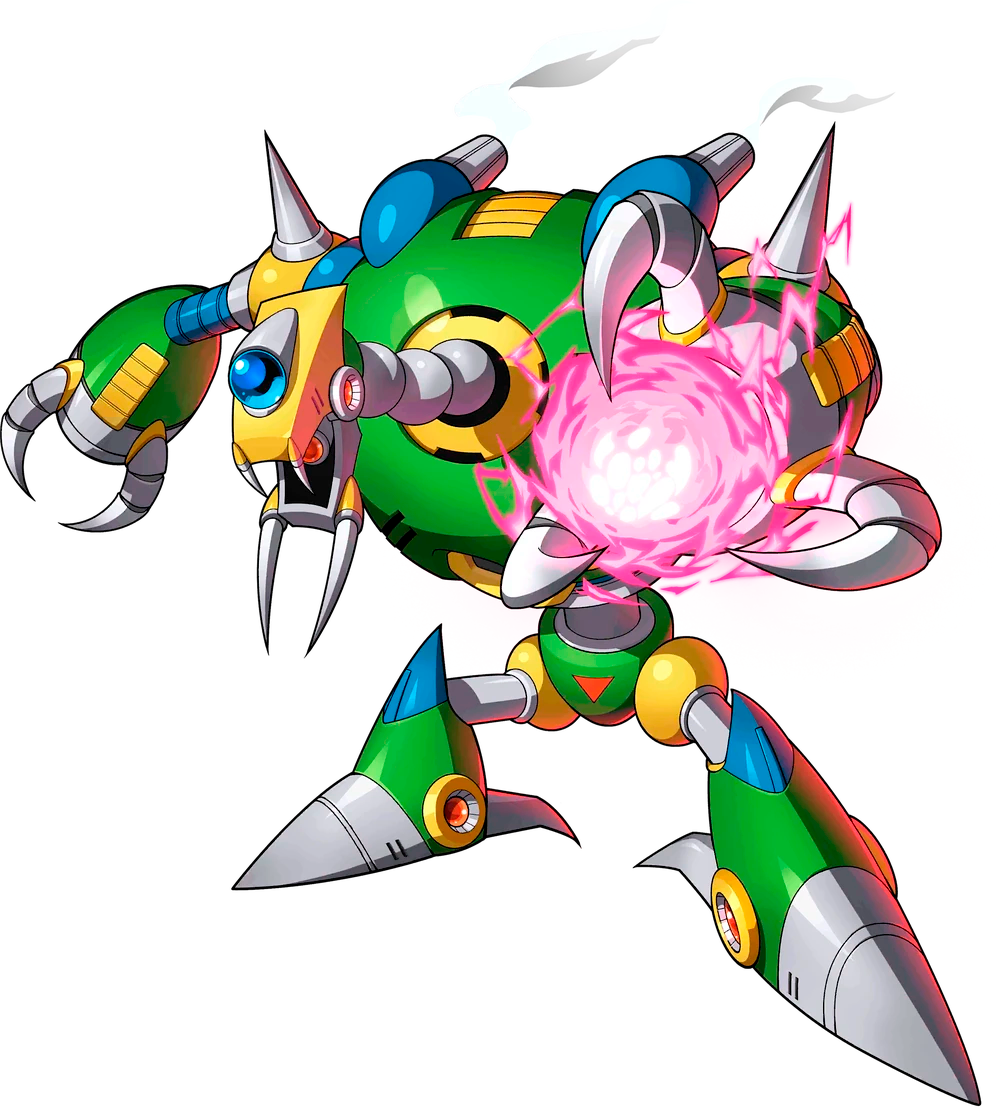
\includegraphics[width=0.3\linewidth]{figures/X2/Enemies/RaiderKiller_Dive.png}
		\caption{Raider Killer's artworks}
	\end{figure}

	\item \hypertarget{miniboss:RT-55J}{\textbf{RT-55J}}: 
	\enemSpecs{64 (0.5 second of Iframes, resist most weapons. Boomerang Cutter deals 3 damage instead of 2)}{2 (contact), 2 (arm)}{In times of peace, it was a professional robot sumo wrestler and a popular Yokozuna (sumo grand champion) in the "Robot Grand Sumo Tournament". Moved in the forest, it now guards X's  Chest Parts. Its certain kill technique, the "Kagizume Beam Hand," strikes and tosses its opponents but only if it is in his claw's reach range. Otherwise he'll just jump at it to close the gap.} 
	\begin{figure}[htp]
		\centering
		
\includegraphics[width=0.3\linewidth]{figures/X1/Enemies/RT-55J.jpg}
		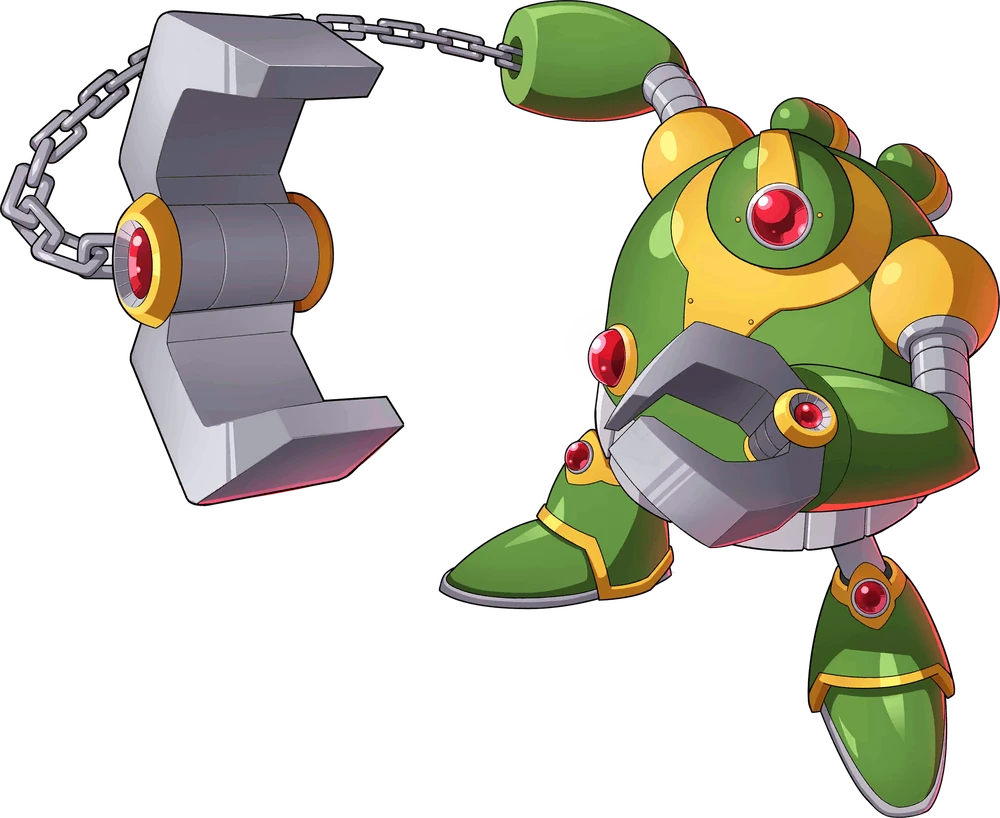
\includegraphics[width=0.5\linewidth]{figures/X1/Enemies/RT55J_Dive.png}
		\caption{RT-55J's artwork}
	\end{figure}
	
	\item \hypertarget{miniboss:Sea_Canthller}{\textbf{Sea Canthller}}
	\enemSpecs{40 (caudal fin), 24 (anal fin), 14 (breast), 10 (pectoral fin), 10 (front dorsal fin), 8 (lower dorsal fin), 4 (eyes), 4 (mouth)~\cite{wiki:Sea_Canthller} }{1 (laser), 3 (contact), 4 (mines)}{Originally, a deep sea working vessel designed as a mother ship for servicing and replenishing the \hyperlink{enem:Jelly_Seeker}{Jelly Seekers}. Now has been remodeled as a transport unit that carries weapons for protecting its cargo.}
	\begin{figure}[htp]%
		\centering
		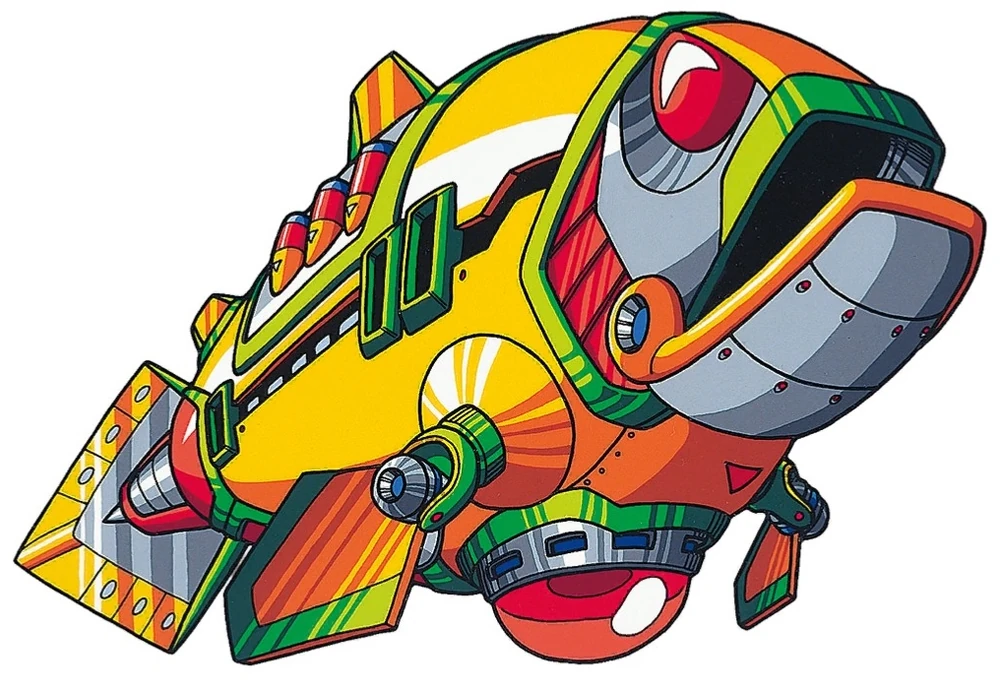
\includegraphics[width=0.4\linewidth]{figures/X2/Enemies/SeaCanthller.png}
		\caption{Sea Canthller's artwork}
	\end{figure}
	
	\item \hypertarget{miniboss:Shurikein}{\textbf{Shurikein}}
	
	
	\item \hypertarget{miniboss:Thunder_Slimer}{\textbf{Thunder Slimer}}: 
	\enemSpecs{48 (0.116 seconds of Iframes, Storm Tornado hits for 9-10 damage)}{5 (contact), 4 (thunders)}{Thunder Slimer was born from a single question: ``How large can a single cell become?'' This monster was born from said experiment. Its body is over three times as large as X, but may require approximately 10 years before it reaches full growth. It has settled in the power plant, where he absorbs electricity and uses it to perform electric attacks against X.}
	\begin{figure}[htp]
		\centering
		
\includegraphics[width=0.3\linewidth]{figures/X1/Enemies/ThunderSlimer.jpg}
		\caption{Thunder Slimer's artwork}
	\end{figure}
	
	\item \hypertarget{miniboss:Utuboros}{\textbf{Utuboros}}: 
	\enemSpecs{72 (no Iframes, Boomerang Cutter hits for 3 damage instead of 2 and Storm Tornado kills it in a single shot)}{4 (contact)}{Serpent-type mechaniloid made to explore the ocean floor. Thanks to its flexible body it can zig-zag into difficult underwater areas, and burrow underground. His body is totally invincible and can work as a platform, while only the head and tail are vulnerable and can damage X.}
	\begin{figure}[htp]
		\centering
		
\includegraphics[width=0.4\linewidth]{figures/X1/Enemies/Utuboros.jpg}
		\caption{Utuboros's artwork}
	\end{figure}
\end{itemize}


\section{Minor enemies}
\begin{itemize}
		
	\item[{
\includegraphics[height=30px]{figures/X2/Enemies/sprite_aclanda.png}}] \hypertarget{enem:Aclanda}{\textbf{Aclanda}}:
	\enemSpecs{16, weak to Silk Shot, Spin Wheel and Magent Mine}{2 (grenades), 3 (laser), 4 (contact)}{Immobile artillery shaped like a scorpion, built by the X-Hunters to intercept the Maverick Hunters.}
	
	\item[{
\includegraphics{figures/X1/Enemies/sprite_amenhopper.png}}] \hypertarget{enem:Amenhopper}{\textbf{Amenhopper}}: 
	\enemSpecs{2}{1 (bombs), 2 (contact)}{Originally designed for farm work, it was used to sow fertilizer 
		across the land. Now, it's been remodeled into a bomb-dropping
		battle type mechaniloid.}

	
	\item[ {
\includegraphics[height=20px]{figures/X1/Enemies/sprite_armor_soldier.png}}] \hypertarget{enem:Armor_Soldier}{\textbf{Armor Soldier}}: 
	\enemSpecs{3 (on foot), 16 (Ride Armor)}{2 (contact, on foot), 3(contact-Armor)}{Lowest class of soldier reploids, used in military affairs. Riding in their Ride Armor, they do destruction work under Sigma's orders.}
	
	\item \hypertarget{enem:Atareeter}{\textbf{Atareeter}} %TODO ---------------------------------------------
	
	\item[{
\includegraphics[width=30px]{figures/X1/Enemies/sprite_axemax.png}}] \hypertarget{enem:Axe_Max}{\textbf{Axe Max}}:
	\enemSpecs{8}{3 (contact, on foot), 2(flying log)}{Woodcutter reploid from the forest, remodeled for brutality. Swinging his large axe, he attacks by sending the chopped wood flying.}
	
	\item[{
\includegraphics[height=20px]{figures/X1/Enemies/sprite_balldevoux.png}}] \hypertarget{enem:Ball_De_Voux}{\textbf{Ball De Voux}}:
	\enemSpecs{2}{1 (contact)}{Equipped with 2 soft-treading feet, this mechaniloid can move over any topography.
		Inside the sphere there is a camera and a sensor which can even see in the dark.}
	
	\item[{
\includegraphics[height=30px]{figures/X2/Enemies/sprite_barwayings.png}}] \hypertarget{enem:Bar_Waying}{\textbf{Bar Waying}}:
	\enemSpecs{9, weak to Silk Shot, Spin Wheel and Magnet Mine}{2 (crush)}{This mechaniloid was developed as a shutter for disaster prevention. Extending its body, it attempts to block the path.}

	
	\item[{
\includegraphics[height=30px]{figures/X2/Enemies/sprite_BariteLastar.png}}] \hypertarget{enem:Barite_Lastar}{\textbf{Barite Lastar}}:
	\enemSpecs{2}{2 (laser), 2 (contact)}{Mechaniroid built for protecting military bases. It moves by attaching itself to a wall and can absorb enemy fire.}
	
	\item[{
\includegraphics[height=30px]{figures/X2/Enemies/sprite_BarrierAttacker.png}}] \hypertarget{enem:Barrier_Attacker}{\textbf{Barrier Attacker}}:
	\enemSpecs{2(must be hit behind the shield)}{2(contact)}{Loading work mechaniloid which equips a barrier for protection.}
	
	\item[{
\includegraphics{figures/X1/Enemies/sprite_battonbone.png}}] \hypertarget{enem:Batton_Bone}{\textbf{Batton Bone}}:
	\enemSpecs{1}{1 (contact)}{Bat mechaniloids with a taste for humans. They dwell in forests and caves.}
	
	\item[{
\includegraphics{figures/X1/Enemies/sprite_battonbone.png}}] \hypertarget{enem:Batton_Bone_type_G}{\textbf{Batton Bone type G}}:
	\enemSpecs{1}{1 (contact)}{Batton Bone like those of the previous production, upgraded with strengthened armor.}
	
	\item[{
\includegraphics[height=15px]{figures/X1/Enemies/sprite_battonm501.png}}]  \hypertarget{enem:Batton_M-501}{\textbf{Batton M-501}}: 
	\enemSpecs{2}{1 (contact)}{Bat type mechaniloid which the \hyperlink{enem:Batton_Bone}{Batton Bone} series is based on. It is a very unusual mechaniloid, made over 30 years ago.}
	
	\item[{
\includegraphics[height=30px]{figures/X2/Enemies/sprite_beetron.png}}] \hypertarget{enem:Beetron}{\textbf{Beetron}}:
	\enemSpecs{16}{4 (contact)}{Beetle type mechaniloid designed for work in the mines.}
	
	\item \hypertarget{enem:Blady}{\textbf{Blady}}%TODO ---------------------------------------------
	
	
	\item[{
\includegraphics[height=30px]{figures/X2/Enemies/sprite_blecker.png}}] \hypertarget{enem:Blecker}{\textbf{Blecker}}:
	\enemSpecs{6}{2 (orbs), 2 (contact)}{Energy cannon which operates during an emergency. When not in operation, this mechaniroid is harmless.}
	
	\item[{
\includegraphics{figures/X1/Enemies/sprite_bombeen.png}}]\hypertarget{enem:Bomb_Been}{\textbf{Bomb Been}}:
	\enemSpecs{2}{2 (contact), 1 (bomb)}{Small bee-modeled helicopter used for land mines scattering. Able to infiltrate any area, it can set up land mines anywhere.}
	
	\item[{
\includegraphics[height=30px]{figures/X2/Enemies/sprite_CannonDriver.png}}] \hypertarget{enem:Cannon_Driver}{\textbf{Cannon Driver}}:
	\enemSpecs{14}{2 (contact), 4 (cannon)}{2-footed walker type interceptor tank. Powerful mechaniloid that fires using two 200 mm cannons and enemy-seeking pursuit missiles.}
	
	\item \hypertarget{enem:Caterkiller}{Caterkiller}	
	
	
	\hyperlink{enem:Carry_Arm}{\textbf{Carry Arm}} (before completing Gravity Beetle's stage)

	
	\item \hypertarget{enem:Crablaster}{\textbf{Crablaster}}%TODO ---------------------------------------------

	
	
	\item[{
\includegraphics[height=20px]{figures/X1/Enemies/sprite_cragman.png}}] \hypertarget{enem:Crag_Man} {\textbf{Crag Man}}:
	\enemSpecs{8}{2 (contact),2 (rock fall)}{Crag Men were made to clear rock debris during landslides. They work actively with the aerial mechaniloid \hyperlink{enem:Sky_Claw}{Sky Claw}.}
	
	\item[{
\includegraphics[height=15px]{figures/X2/Enemies/sprite_CrashRoader.png}}] \hypertarget{enem:Crash_Roader}{\textbf{Crash Roader}}:
	\enemSpecs{3}{2 (contact)}{Member of a gang rival of the \hyperlink{enem:Road_Attackers}{Road Attackers}. Once they start rolling, they won't turn until they hit a wall}
	
	\item[{
\includegraphics[height=10px]{figures/X1/Enemies/sprite_creeper.png}}] \hypertarget{enem:Creeper} {\textbf{Creeper}}:
	\enemSpecs{1}{1 (contact)}{An insect-type mechaniloid. It's unknown what it was made for.	It is pecked out from the insides of trees by the \hyperlink{enem:Mad_Pecker}{Mad Pecker}.}
	
	\item[{
\includegraphics[height=20px]{figures/X2/Enemies/sprite_CroakHopper.png}}] \hypertarget{enem:Croak_hopper}{\textbf{Croak Hopper}}:
	\enemSpecs{4}{1 (shots), 3 (contact)}{Once the mascots of the Weather Control Center, were later remodeled by the X-Hunters for attack.}
	
	\item[{
\includegraphics[height=20px]{figures/X1/Enemies/sprite_crusher.png}}] \hypertarget{enem:Crusher}{\textbf{Crusher}}:
	\enemSpecs{2}{4}{Construction mechaniloid used for knocking down buildings. It drops its steel-made weight to scrape down the highway.}
	
	\item[{
\includegraphics[height=20px]{figures/X1/Enemies/sprite_diglabour.png}}] \hypertarget{enem:Dig_Labour}{\textbf{Dig Labour}}: 
	\enemSpecs{4}{2(pickaxe), 3(contact)}{The greatest pickaxe worker in the world. He is a diligent reploid who works in the robot factory.}
	
	\item[{
\includegraphics[height=20px]{figures/X2/Enemies/sprite_DiskBoy08.png}}] \hypertarget{enem:Disk_Boy_08}{\textbf{Disk Boy 08}}:
	\enemSpecs{6}{2 (disc), 2 (contact)}{Reploid player of the combat sport "Snapper Disk", model number 8.}
	
	\item[{
\includegraphics[height=20px]{figures/X1/Enemies/sprite_dodgeblaster.png}}] \hypertarget{enem:Dodge_Blaster}{\textbf{Dodge Blaster}}: 
	\enemSpecs{3}{2 (contact), 2(shots)}{Latest model of mobile cannon with "self-defense function", which makes it possible to avoid energy attacks before they can even get near it.}
	
	\item \hypertarget{enem:Drimole-W }{\textbf{Drimole-W} }%TODO ---------------------------------------------

	\item \hypertarget{enem:Earth_Commander}{\textbf{Earth Commander}}%TODO ---------------------------------------------
	
	\item[{
\includegraphics[height=15px]{figures/X2/Enemies/sprite_Fishern.png}}] \hypertarget {enem:Fishern}{\textbf{Fishern}}:
	\enemSpecs{1}{1 (contact)}{Formerly a mechaniloid for feeding cultivated fish. After being remodeled, it breaks everything in sight.}
	
	\item[{
\includegraphics[height=20px]{figures/X1/Enemies/sprite_flamer.png}}] \hypertarget{enem:Flamer}{\textbf{Flamer}}:
	\enemSpecs{6}{3 (contact), 2(fire)}{High-temperature blaze-blowing flamethrower machine. A remodeled airport fire extinguisher mechaniloid, turned into a weapon which tries to spread fires.}
	
	\item[{
\includegraphics[height=30px]{figures/X1/Enemies/sprite_flammingle.png}}] \hypertarget{enem:Flammingle}{\textbf{Flammingle}}:
	\enemSpecs{8, 4 (saw)}{3 (contact), 2(blade)}{Flamingo-type mechaniloid taken from the robot zoo. It attacks by spinning its head and releasing the saw.}
	
	\item \hypertarget{enem:Ganseki_Carrier}{\textbf{Ganseki Carrier}}%TODO ---------------------------------------------
	
	
	\item[{
\includegraphics[height=30px]{figures/X2/Enemies/sprite_GarakutaRobot.png}}] \hypertarget{enem:Garakuta_Robot}{\textbf{Garakuta Robot}}:
	\enemSpecs{8 (can regenerate broken parts, Silk Shot instantly kill)}{1 (contact)}{Ghastly mechaniloids made from broken \hyperlink{enem:Metall_C-15}{Metall}, \hyperlink{enem:Dig_Labour}{Dig Labours}, \hyperlink{enem:Gulpfer}{Gulpfers} and \hyperlink{enem:Spiky}{Spikys}}.
	
	\item[{
\includegraphics[height=20px]{figures/X1/Enemies/sprite_gulpfer.png}}] \hypertarget{enem:Gulpfer}{\textbf{Gulpfer}}:
	\enemSpecs{10}{2 (contact), 2-32 (eating)}{Once the ornamental mascot mechaniloid of a seaside Chaya teahouse, it escaped and was converted for catching ocean fish. It was originally based on an old children's toy.}
	
	\item[{
\includegraphics[height=20px]{figures/X1/Enemies/sprite_gunvolt.png}}] \hypertarget{enem:Gun_Volt}{\textbf{Gun Volt}}:
	\enemSpecs{16}{3 (contact), 2(sparks), 2(missiles)}{Mechaniloid developed for military use. A tank made for terrestrial combat, it attacks with missiles and high voltage bullets.}
	
	\item \hypertarget{enem:Hamma_Hamma}{\textbf{Hamma Hamma}}%TODO ---------------------------------------------
	
	
	
	\item[{\includegraphics[height=30px]{figures/X2/Enemies/sprite_HangedReploid.png}}] \hypertarget{enem:Hanged_Reploid}{\textbf{Hanged Reploid}}:
	\enemSpecs{1(head), 3(Body)}{2 (fireballs), 2(contact)}{Pitiful reploid left in the scrap processing yards. Will attack and try to cling to anything that approaches.}
	
	\item \hypertarget{enem:Hangerter}{Hangerter}
	
		
	\item \hypertarget{enem:Head_Gunner_customer}{\textbf{Head Gunner customer}} %TODO ---------------------------------------------
	\item \hypertarget{enem:Head_Gunner_masspro}{\textbf{Head Gunner masspro}}%TODO ---------------------------------------------
	
	\item \hypertarget{enem:Helit}{\textbf{Helit}}%TODO ---------------------------------------------
	
	\item[{\includegraphics[height=20px]{figures/X1/Enemies/sprite_hoganmer.png}}] \hypertarget{enem:Hoganmer}{\textbf{Hoganmer}}:
	\enemSpecs{8}{3 (contact), 2(spike ball)}{Fighter in the future grappling show "Robot Coliseum." It blocks the attacks of enemies with its shield, and attacks	by swinging its iron ball and chain.}
	
	\item[{\includegraphics[height=20px]{figures/X1/Enemies/sprite_hotarion.png}}] \hypertarget{enem:Hotarion}{\textbf{Hotarion}}:
	\enemSpecs{1}{2 (contact)}{A mechaniloid for nighttime patrol, it was made to save the firefly appearance from extinction. Shining, it flies through the sky.}
	
	
	\item \hypertarget{enem:Ice_De_Voux}{\textbf{Ice De Voux}}  %TODO ---------------------------------------------
	
	
	\item[{\includegraphics[height=30px]{figures/X2/Enemies/sprite_Installer.png}}] \hypertarget{enem:Installer}{\textbf{Installer}}:
	\enemSpecs{7}{Insta-kill (crush)}{Large mobile equipment which perform maintenance in the Computer Center.}
	
	\item[{\includegraphics[height=20px]{figures/X1/Enemies/sprite_jamminger.png}}] \hypertarget{enem:Jamminger}{\textbf{Jamminger}}:
	\enemSpecs{2}{1 (contact)}{Mechaniloid that attacks any enemies who enter a forbidden area. An odd robot who laughs after attacking.}
	
	\item[{\includegraphics[height=20px]{figures/X2/Enemies/sprite_JellySeeker.png}}] \hypertarget{enem:Jelly_Seeker}{\textbf{Jelly Seeker}}:
	\enemSpecs{2}{2 (contact)}{Mechanloid for deep sea exploration. In order to withstand the water pressure, it has an outer jelly-like layer. It also has a function to generate electricity on its own.}
	
	\item[{\includegraphics[height=20px]{figures/X1/Enemies/sprite_ladderyadder.png}}] \hypertarget{enem:Ladder_Yadder}{\textbf{Ladder Yadder}}:
	\enemSpecs{3}{2 (contact)}{Originally a mechaniloid supervisor of the forest regions. It would locate any poachers, and report the forest's temperature and humidity to the woodland protection center.}
	
	\item[{\includegraphics[height=20px]{figures/X1/Enemies/sprite_liftcannon.png}}] \hypertarget{enem:Lift_Cannon}{\textbf{Lift Cannon}}:
	\enemSpecs{2}{3(contact), 2(shot)}{Rotary-type cannon attached to a tube-like stand. Originally, a fire-fighting robot for control towers and any other high places in the airport.}
	
	\item[{\includegraphics[height=20px]{figures/X1/Enemies/sprite_madpecker.png}}] \hypertarget{enem:Mad_Pecker}{\textbf{Mad Pecker}}:
	\enemSpecs{6}{2 (contact)}{Woodpecker-type repliroid who chops trees in the forest. Tries to follow \hyperlink{enem:Planty_Iworms}{Planty}, without success.}
	
	\item[{\includegraphics[height=30px]{figures/X2/Enemies/sprite_MechaArm.png}}] \hypertarget{enem:Mecha-Arm}{\textbf{Mecha-Arm}}:
	\enemSpecs{-}{-}{Robot installed in the automation system in the mechaniloid factory.}
	
	\item[{\includegraphics[width=30px]{figures/X1/Enemies/sprite_megatortoise.png}}] \hypertarget{enem:Mega_Tortoise}{\textbf{Mega Tortoise}}:
	\enemSpecs{16}{4(contact),3 (bombs)}{A turtle-type mechaniloid originally meant for rescuing humans from maritime disasters. From its back, it now produces bombs in place of floating devices.}
	
	\item \hypertarget{enem:Meta_Capsule}{\textbf{Meta Capsule}}%TODO ---------------------------------------------
	
	
	\item[{\includegraphics{figures/X1/Enemies/sprite_metalwing.png}}] \hypertarget{enem:Metal_Wing}{\textbf{Metal Wing}}: 
	\enemSpecs{1}{3 (contact)}{A reconnaissance mechaniloid. When it spots dangers, it raises its flying speed in a great rush to get news to its master.}
	
	\item[{\includegraphics{figures/X1/Enemies/sprite_mettalc15.png}}] \hypertarget{enem:Metall_C-15}{\textbf{Metall C-15}}: 
	\enemSpecs{2}{2 (contact), 1(bullet)}{Reploid who watches factories. From the former series that worked in factories, now they are advanced enough to be placed as chiefs.}
	
	 \hypertarget{enem:Mine_Tortoise}{\textbf{Mine Tortoise}}%TODO ---------------------------------------------

	
	\item[{\includegraphics[height=30px]{figures/X2/Enemies/sprite_Morgun.png}}] \hypertarget{enem:Morgun}{\textbf{Morgun}}:
	\enemSpecs{1}{1 (contact), 3 (fireballs)}{Mechaniloid for geological surveying, its body is designed to withstand the heat and pressure of hot magma}
	
	\item \hypertarget{enem:Notor_Banger}{\textbf{Notor Banger}}%TODO ---------------------------------------------
	

	
	
	\item[{\includegraphics[height=20px]{figures/X2/Enemies/sprite_pararoid.png}}] \hypertarget{enem:Pararoid_R-5}{\textbf{Pararoid R-5}}:
	\enemSpecs{2}{2 (contact)}{Pararoid model improved with the ability of flight. It can approach suddenly by dashing at super speed.}
	
	\item[{\includegraphics[height=10px]{figures/X2/Enemies/sprite_pararoidv1.png}}] \hypertarget{enem:Pararoid_V-1}{\textbf{Pararoid V-1}}:
	\enemSpecs{2}{2 (contact, can attach to X's head and force him to continuously dash, shoot or jump. Can be de-attached by mashing buttons)}{Mechaniloid with the ability to short-circut scrapped mechaniloids and reploids and turn them into mavericks. It can also attach to living reploids and temporarily corrupt their motion circuits.}
	
	\item[{\includegraphics{figures/X1/Enemies/sprite_planty.png}}] \hypertarget{enem:Planty_Iworms} {\textbf{Planty\&Iworms}}: 
	\enemSpecs{2 (Planty), 1 (Iworm)}{3 (contact-Planty), 1(contact-Iworm)}{Planty is from the Mettool family and watches over the forest. From its head, it can manufacture the earthworm-type, soil cultivation reploid, Iworm.}
	
	\item[{\includegraphics{figures/X1/Enemies/sprite_raybit.png}}] \hypertarget{enem:Ray_Bit}{\textbf{Ray Bit}}: 
	\enemSpecs{2}{4 (contact), 3 (laser)}{Rabbit-type mechaniloid taken from the robot zoo. It skips and jumps, using the laser cannon in its ears to attack.}
	
	\item[{\includegraphics[height=15px]{figures/X1/Enemies/sprite_raytrap.png}}] \hypertarget{enem:Ray_Trap}{\textbf{Ray Trap}}: 
	\enemSpecs{-}{-}{Mechaniloid devices which await the false steps of intruders.}
	
	\item[{\includegraphics[height=20px]{figures/X2/Enemies/sprite_Refleczer.png}}] \hypertarget{enem:Refleczer}{\textbf{Refleczer}}:
	\enemSpecs{2}{1 (bullets), 2 (contact)}{Defensive artillery. Its laser is refracted by the crystal, so that it can attack enemies in several directions.}
	
	\item[{\includegraphics[height=30px]{figures/X2/Enemies/sprite_RideloidG.png}}] \hypertarget {enem:Rideroid G}{\textbf{Rideroid G}}:
	\enemSpecs{1 (on foot), 16 (with armor)}{3 (contact), 4 (punch)}{Reploid soldier in training to use the RABBIT Ride Armor. Still undergoing training, it is not very strong.}
	
	\item[{\includegraphics[height=30px]{figures/X2/Enemies/sprite_Rightod.png}}] \hypertarget{enem:Rightod}{\textbf{Rightod}}:
	\enemSpecs{1}{4 (lightning)}{Hatched from the capsule weapon number one dropped by Sky Farmers. They fly and attach to the enemy, then attack by calling upon thunder.}
	
	\item[{\includegraphics[width=30px]{figures/X1/Enemies/sprite_roadattacker.png}}] \hypertarget{enem:Road_Attackers}{\textbf{Road Attackers}}: 
	\enemSpecs{12(total), at 7/12 the pilot dies; at 3/12 the engine explodes}{2 (contact), 1 (shot)}{A destructive reploid gang of hot-rodders, riding for Sigma's rebellion. Large beam cannons have been attached to the bonnets of their sports cars.}
	
	\item[{\includegraphics[height=20px]{figures/X2/Enemies/sprite_RideChaserCheval.png}}] \hypertarget{enem:Road_Riders}{\textbf{Road Riders}}:
	\enemSpecs{3}{2 (contact), 3 (bombs)}{Members of a Robot gang of hot-rodders. Formerly, they blasted the town during the night and ran off. They love to drive the Ride Chaser.}
	
	\item[{\includegraphics{figures/X1/Enemies/sprite_rollinggabyoall.png}}] \hypertarget{enem:Rolling_Gabyoall}{\textbf{Rolling Gabyoall}}: 
	\enemSpecs{1 (Immune to all but Rolling Shield)}{3 (contact)}{Intruder repulsion robot. It Appears to be a simple mechaniloid, but truthfully, it possesses the human-like mind of a reploid.}
	
	\item[{\includegraphics{figures/X1/Enemies/sprite_rushroader.png}}] \hypertarget{enem:Rush_Roader}{\textbf{Rush Roader}}: 
	\enemSpecs{6}{2 (contact)}{Leaders of the robot gang of hot-rodders. To get revenge on the Maverick Hunters who once chased them down, they became Sigma's subordinate.}
	
	\item[{\includegraphics[height=30px]{figures/X2/Enemies/sprite_Sabottein.png}}] \hypertarget{enem:Sabottein}{\textbf{Sabottein}}:
	\enemSpecs{7}{2 (contact)}{Capsule weapon number 2, it was designed as a mecha for aiding in affecting the atmosphere in the Weather Control Center.}
	
	\item[{\includegraphics[height=20px]{figures/X2/Enemies/sprite_scrambler.png}}] \hypertarget{enem:Scrambler}{\textbf{Scrambler}}:
	\enemSpecs{1}{1 (contact)}{Flying battle mechaniloid which attacks by extending its cutter arms. Its thin armor helps to guarantee mobility, but it is also its weakness}
	
	\item[{\includegraphics[height=20px]{figures/X1/Enemies/sprite_scraprobo.png}}] \hypertarget{enem:Scrap_Robo}{\textbf{Scrap Robo}}:
	\enemSpecs{4}{3 (contact), 2(laser))}{A pathetic upper body of a robot, made to become a car driver. Although it passed part of the humans' expectations, without a driver's license, it has been turned into scrap.}
	
	\item[{\includegraphics[height=10px]{figures/X2/Enemies/sprite_scriver.png}}] \hypertarget{enem:Scriver}{\textbf{Scriver}}:
	\enemSpecs{2}{2 (contact)}{Originally an assembly worker mechaniloid for manufacturing jobs in the factory, but was later remodeled for attack.}
	
	\item[{\includegraphics[height=20px]{figures/X1/Enemies/sprite_seaattacker.png}}] \hypertarget{enem:Sea_Attacker}{\textbf{Sea Attacker}}:
	\enemSpecs{2}{2 (contact)}{Seahorse-type mechaniloid created as a novelty for humans' homes. Its body somersaults as it charges.}
	
	\item[{\includegraphics{figures/X1/Enemies/sprite_sinefaller.png}}] \hypertarget{enem:Sine_Faller}{\textbf{Sine Faller}}:
	\enemSpecs{1}{2 (contact)}{Aerial mechaniloid made with the idea "Quality from quantity". It flies and turns, acting as a hindrance.}
	
	\item[{\includegraphics[height=20px]{figures/X1/Enemies/sprite_skyclaw.png}}] \hypertarget{enem:Sky_Claw}{\textbf{Sky Claw}}:
	\enemSpecs{2}{2 (contact), 3(self-destruct)}{A robot who removes obstacles, originally designed for the ``Crane Game'' which was popular in Japan during the later half of the twentieth century.}
	
	\item[{\includegraphics[height=30px]{figures/X2/Enemies/sprite_SkyFarmer.png}}] \hypertarget{enem:Sky_farmer}{\textbf{Sky Farmer}}:
	\enemSpecs{2}{1 (capsule weapon), 2 (contact)}{Mechaniloid made for sowing seeds from the air, remodeled to drop capsule weapons.}
	
	\item[{\includegraphics[height=20px]{figures/X2/Enemies/sprite_slidame.png}}] \hypertarget{enem:Slidame}{\textbf{Slidame}}:
	\enemSpecs{2}{2 (contact), close walls for insta-kill}{Flying patrol mechaniloid which closes the shutter when an enemy gets close.}
	
	\item[{\includegraphics[width=30px]{figures/X1/Enemies/sprite_slidecannon.png}}] \hypertarget{enem:Slide_Cannon}{\textbf{Slide Cannon}}:
	\enemSpecs{3}{2 (contact), 2(shot)}{Defensive artillery, set up to attack aerial enemies. Designed after the German anti-aircraft cannons of the 1940s.}
	
	\item[{\includegraphics[height=20px]{figures/X1/Enemies/sprite_snowshooter.png}}] \hypertarget{enem:Snow_Shooter}{\textbf{Snow Shooter}}: 
	\enemSpecs{4}{3 (contact), 2(snowball)}{Bad-natured mechaniloid who toss balls of white iron as if they were snowballs. They are Chill Penguin's guardians.}
	
	\item \hypertarget{enem:Snow_Rider}{\textbf{Snow Rider}}  %TODO ---------------------------------------------
	\item \hypertarget{enem:Snow_Slider}{\textbf{Snow Slider}} %TODO ---------------------------------------------
	
	
	\item[{\includegraphics[height=30px]{figures/X2/Enemies/sprite_SoleSolar.png}}] \hypertarget{enem:Sole_solar}{\textbf{Sole Solar}}:
	\enemSpecs{3}{2 (missiles), 5 (laser)}{Artillery robots of the Weather Control Center, which runs off sunlight. There are 2 types. The L type fire lasers, while the M type are equipped with pursuit missiles}
	
	\item[{\includegraphics[height=20px]{figures/X1/Enemies/sprite_spiky.png}}] \hypertarget{enem:Spiky}{\textbf{Spiky}}: 
	\enemSpecs{2}{2 (contact)}{Monocycle which bears sharp spikes in its tire. Very dangerous, its main attack technique is to slide over and self-destruct.}
	
	\item[{\includegraphics[height=20px]{figures/X2/Enemies/sprite_tiranos.png}}] \hypertarget {enem:Tiranos}{\textbf{Tiranos}}:
	\enemSpecs{3}{2 (cannon), 2(contact)}{A small-sized tank for guarding restricted areas. Originally an exhibit at the dinosaur robot museum.}
	
	\item[{\includegraphics{figures/X1/Enemies/sprite_tombot.png}}] \hypertarget{enem:Tombot}{\textbf{Tombot}}:
	\enemSpecs{1}{2 (contact)}{A dragonfly-type glider. When taking off, it cuts and releases the jet propulsion units. Then, slowly riding the wind, it flies through the sky.}
	
	\item \hypertarget{enem:Tombort}{\textbf{Tombort}}%TODO ---------------------------------------------
	
	\item[{\includegraphics[height=10px]{figures/X2/Enemies/sprite_TubamailGenerator.png}}] \hypertarget {enem:Tubamail_Generator}{\textbf{Tubamail Generator}}:
	\enemSpecs{8}{2 (contact)}{Platform which constructs and releases Tubamail-S.}
	
	\item[{\includegraphics[height=20px]{figures/X2/Enemies/sprite_Tubamail-s.png}}] \hypertarget {enem:Tubamail-S}{\textbf{Tubamail-S}}
	\enemSpecs{2}{1 (contact)}{High speed mechaniloid originally designed for carrying the mail, now remodeled as suicidal missile attackers.}
	
	\item[{\includegraphics[width=20px]{figures/X1/Enemies/sprite_turncannon.png}}] \hypertarget{enem:Turn_Cannon}{\textbf{Turn Cannon}}: 
	\enemSpecs{5}{}{Robot once designed as a sprinkler for domestic use, but was defective until the water was replaced with cannon shells.}
	
	\item \hypertarget{enem:Victoroid}{\textbf{Victoroid}} %TODO ---------------------------------------------

	\item \hypertarget{enem:Victoroid_customer}{\textbf{Victoroid customer}}%TODO ---------------------------------------------

	\item \hypertarget{enem:Walk Blaster}{\textbf{Walk Blaster}}%TODO ---------------------------------------------
	
	\item \hypertarget{enem:Wall_Cancer}{\textbf{Wall Cancer}} %TODO ---------------------------------------------
	
	
	\item[{\includegraphics[height=20px]{figures/X2/Enemies/sprite_weathercrystal.png}}] \hypertarget{enem:Weather_crystal}{\textbf{Weather Crystal}}:
	\enemSpecs{22}{-}{Device which creates and maintains the artificial weather inside the Weather Control Center. Because it is such a precision instrument, it has a fault which makes it easily affected by outside stimulus.}

	
\end{itemize}











